% !TEX TS-program = pdflatex
% CV — Baha Eddine Belhaj Mouldi — one-page professional layout (English)
\documentclass[a4paper,10pt]{article}
\usepackage[utf8]{inputenc}
\usepackage[T1]{fontenc}
\usepackage{lmodern}
\usepackage[left=1.1cm,right=1.1cm,top=1.0cm,bottom=0.9cm]{geometry}
\usepackage{enumitem}
\usepackage{xcolor}
\usepackage{amssymb}
\usepackage{titlesec}
\usepackage{tikz}
\usepackage{graphicx}
\usepackage{marvosym}
\usepackage{paracol}
\usepackage[hidelinks]{hyperref}
\definecolor{accent}{RGB}{0,90,170}
\definecolor{accentlight}{RGB}{0,120,215}
\definecolor{darktext}{RGB}{34,40,49}
\definecolor{graytext}{RGB}{90,98,110}
\definecolor{rulegray}{RGB}{215,219,225}
\renewcommand{\familydefault}{\sfdefault}
\color{darktext}
\setlength{\parindent}{0pt}
\setlength{\parskip}{0pt}
\linespread{1.02}
\pagestyle{empty}
\titleformat{\section}
  {\large\bfseries\color{accent}}{}{0pt}
  {}[{\vspace{1pt}\color{rulegray}\titlerule[1pt]}]
\titlespacing*{\section}{0pt}{8pt}{5pt}
\setlist[itemize]{leftmargin=1.1em,label=\textcolor{accent}{\small$\blacktriangleright$},
  itemsep=1.2pt,topsep=2pt,parsep=0pt,labelsep=0.5em}
\newcommand{\role}[3]{%
  {\bfseries #1}\hfill{\small\color{graytext}#2}\\[1pt]
  {\itshape\small\color{accentlight}#3}\par\vspace{2pt}}
\newcommand{\skillcat}[2]{%
  {\bfseries\color{darktext}#1}\\[1pt]{\small\color{graytext}#2}\par\vspace{5pt}}
\newcommand{\contactitem}[2]{\textcolor{accent}{#1}~#2}
\begin{document}
\begin{minipage}[c]{0.75\textwidth}
  {\fontsize{24}{26}\selectfont\bfseries\color{darktext}BAHA EDDINE BELHAJ MOULDI}\\[3pt]
  {\large\color{accent}Cybersecurity \& AI Engineer}\\[7pt]
  {\small
    \contactitem{\Telefon}{\href{tel:+21655128982}{+216 55 128 982}}\quad
    \contactitem{\Letter}{\href{mailto:bahaeddine.belhajmouldi@gmail.com}{bahaeddine.belhajmouldi@gmail.com}}\\[3pt]
    \contactitem{\textbf{in}}{\href{https://www.linkedin.com/in/bahamouldi}{linkedin.com/in/bahamouldi}}\quad
    \contactitem{\textbf{GitHub}}{\href{https://github.com/bahamouldi}{github.com/bahamouldi}}\quad
    \contactitem{\textbf{$\bullet$}}{Tunis, Tunisia}
  }
\end{minipage}\hfill
\begin{minipage}[c]{0.22\textwidth}
  \raggedleft
  \begin{tikzpicture}
    \clip (0,0) circle (1.25cm);
    \node at (0,0) {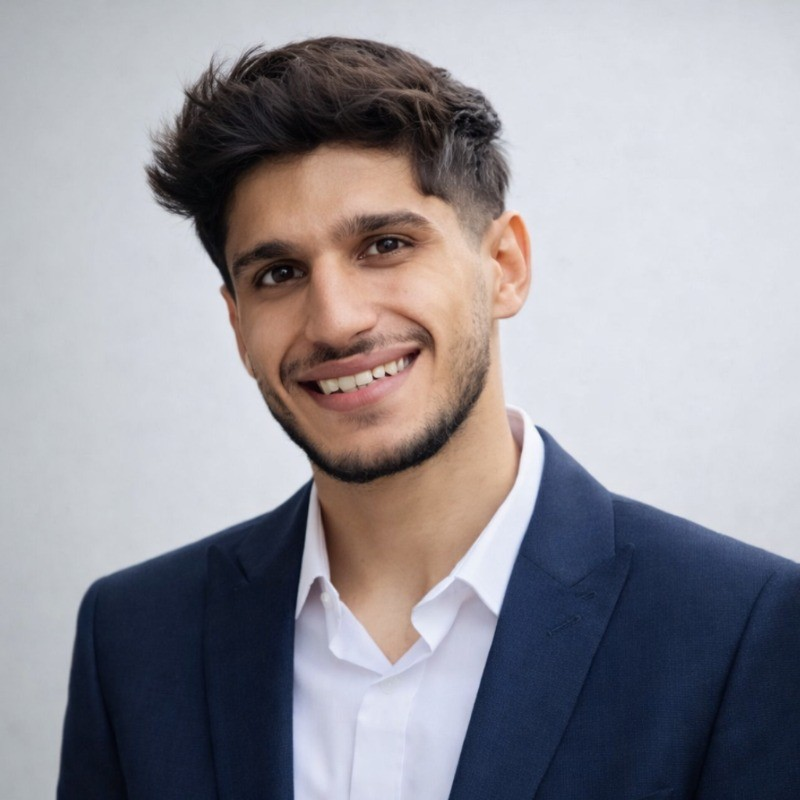
\includegraphics[width=2.6cm,height=2.6cm,keepaspectratio]{photo.jpg}};
    \draw[accent,line width=1.5pt] (0,0) circle (1.24cm);
  \end{tikzpicture}
\end{minipage}
\vspace{4pt}
\noindent\textcolor{accent}{\rule{\linewidth}{1.5pt}}
\vspace{2pt}
\columnratio{0.34}
\setlength{\columnsep}{1.4em}
\begin{paracol}{2}
\section*{}
\vspace{-14pt}
\section{Skills}
\skillcat{Offensive Security}{Web \& API Pentest, OWASP Top 10, XSS, SQLi, CSRF, fuzzing, MITM, Wi-Fi security}
\skillcat{Security Tools}{Burp Suite, OWASP ZAP, Metasploit, Nmap, Wireshark, Hydra, Ettercap}
\skillcat{AI \& Machine Learning}{Python, Scikit-learn, Pandas, K-Means, Adversarial ML (FGSM/PGD), SHAP, LLM/RAG, LangChain}
\skillcat{DevSecOps \& Cloud}{Docker, Kubernetes, CI/CD, Jenkins, GitHub Actions, ELK Stack, Prometheus}
\skillcat{Data \& Systems}{MySQL, MongoDB, Kali Linux, Bash, PowerShell, Git}
\skillcat{Secure Coding}{OWASP best practices, encryption (AES, SHA), access management}
\section{Languages}
\begin{itemize}
  \item English — B2
  \item French — B2
  \item Chinese — Basic
\end{itemize}
\section{Certifications}
\begin{itemize}
  \item Fundamentals of Deep Learning — \textbf{NVIDIA} (2025)
  \item Exploring Adversarial ML — \textbf{NVIDIA} (2025)
  \item Machine Learning — \textbf{NVIDIA} (2024)
  \item Networking — \textbf{Cisco} (2025)
  \item Git \& GitHub — \textbf{365 Data Science} (2024)
\end{itemize}
\switchcolumn
\section{Profile}
{\small Computer engineering graduate from ENIT, specialized in \textbf{offensive cybersecurity} and \textbf{AI applied to security}. Hands-on experience in penetration testing, ML-based attack detection and multi-agent architectures. Seeking a junior position in application security or AI engineering.}
\section{Education}
\role{National Engineering School of Tunis (ENIT)}{2023 -- 2026}{Engineering Degree in Computer Science — graduated 25/06/2026}
\role{Preparatory Institute for Engineering Studies, El Manar}{2021 -- 2023}{Physics \& Technology — ranked 65\textsuperscript{th}/600+ in national exam}
\role{Lycée Abdelaziz Khouja, Kélibia}{2021}{Technical Baccalaureate — High Distinction}
\section{Experience}
\role{Intern — SAP Threat Detection}{Jul. -- Aug. 2025}{Streamlink, Tunisia}
\begin{itemize}
  \item Real-time prototype for detecting suspicious activities on SAP systems.
  \item Automated collection via Python/PyRFC and event correlation in ELK.
\end{itemize}
\role{Intern — Network Security}{Jul. 2024}{Tunisie Telecom, Tunisia}
\begin{itemize}
  \item Network security assessment: 10+ vulnerabilities identified.
  \item Partial test automation (Python \& Bash scripts).
\end{itemize}
\role{Technical Project Lead — Vmate}{Jun. 2024}{ENIT, Tunisia}
\begin{itemize}
  \item Led team of 4 on secure web/mobile platform — \textbf{project ranked 1\textsuperscript{st}}.
\end{itemize}
\section{Technical Projects}
\role{BeeWAF — Intelligent Web Application Firewall (Final-Year Project)}{2026}{FastAPI, ML, Docker, Kubernetes, ELK}
\begin{itemize}
  \item Enterprise WAF: 10,041 rules + 3 ML models (RandomForest, GradientBoosting, IsolationForest) — score 98.2/100, 0\% false positives.
  \item 27 modules: anti-bot, DLP, anti-DDoS, virtual patching (37 CVEs), compliance with 7 frameworks (OWASP, PCI DSS, GDPR, NIST, ISO 27001\dots).
\end{itemize}
\role{Web Attack Detection via Data Mining}{2024}{Python, Scikit-learn, SHAP, AWS}
\begin{itemize}
  \item K-Means clustering pipeline (silhouette 0.787) on AWS logs: 39 attacks detected (13.8\% of traffic).
\end{itemize}
\role{WebSec — Web Security Testing Platform (PFA2)}{2025}{Python, OWASP ZAP}
\begin{itemize}
  \item Automated web vulnerability testing (XSS, SQLi) with report generation.
\end{itemize}
\end{paracol}
\end{document}
